\section{Related rates} \label{S:3.1.RelatedRates}

\begin{goals}
\item If two quantities that are related, such as the radius and volume of a spherical balloon, are both changing as implicit functions of time, how are their rates of change related?  That is, how does the relationship between the values of the quantities affect the relationship between their respective derivatives with respect to time?
\end{goals} 

%--------------------------------------
% SUBSECTION INTRODUCTION
%--------------------------------------
\subsection*{Introduction}

In most of our study of derivatives so far, we have worked in settings where one quantity (often called $y$) depends explicitly on another (say $x$), and in some way we have been interested in the instantaneous rate at which $y$ changes with respect to $x$, leading us to compute $\frac{dy}{dx}$.  These settings emphasize how the derivative enables us to quantify how the quantity $y$ is changing as $x$ changes at a given $x$-value.

We are next going to consider situations where multiple quantities are related to one another and changing, but where each quantity can be considered an implicit function of the variable $t$, which represents time.  Through knowing how the quantities are related, we will be interested in determining how their respective rates of change with respect to time are related.  For example, suppose that air is being pumped into a spherical balloon in such a way that its volume increases at a constant rate of $20$ cubic inches per second.  It makes sense that since the balloon's volume and radius are related, by knowing how fast the volume is changing, we ought to be able to relate this rate to how fast the radius is changing.  More specifically, can we find how fast the radius of the balloon is increasing at the moment the balloon's diameter is $12$ inches?

The following preview activity leads you through the steps to answer this question.

\begin{pa} \label{PA:3.5}
A spherical balloon is being inflated at a constant rate of $20$ cubic inches per second.  How fast is the radius of the balloon changing at the instant the balloon's diameter is $12$ inches?  Is the radius changing more rapidly when $d = 12$ or when $d = 16$?  Why?
\ba
	\item Draw several spheres with different radii, and observe that as volume changes, the radius, diameter, and surface area of the balloon also change.  
	\item Recall that the volume of a sphere of radius $r$ is $V = \frac{4}{3} \pi r^3$.  Note well that in the setting of this problem, \emph{both} $V$ and $r$ are changing as time $t$ changes, and thus both $V$ and $r$ may be viewed as implicit functions of $t$, with respective derivatives $\frac{dV}{dt}$ and $\frac{dr}{dt}$.  
	
	Differentiate both sides of the equation $V = \frac{4}{3} \pi r^3$ with respect to $t$ (using the chain rule on the right) to find a formula for $\frac{dV}{dt}$ that depends on both $r$ and $\frac{dr}{dt}$.
	\item At this point in the problem, by differentiating we have ``related the rates'' of change of $V$ and $r$.  Recall that we are given in the problem that the balloon is being inflated at a constant \emph{rate} of $20$ cubic inches per second.  Is this rate the value of $\frac{dr}{dt}$ or $\frac{dV}{dt}$?  Why?
	\item From part (c), we know the value of $\frac{dV}{dt}$ at every value of $t$.  Next, observe that when the diameter of the balloon is $12$, we know the value of the radius.  In the equation $\frac{dV}{dt} = 4\pi r^2 \frac{dr}{dt}$, substitute these values for the relevant quantities and solve for the remaining unknown quantity, which is $\frac{dr}{dt}$.  How fast is the radius changing at the instant $d = 12$?
	\item How is the situation different when $d = 16$?  When is the radius changing more rapidly, when $d = 12$ or when $d = 16$?
\ea
\end{pa} 
\afterpa % PREVIEW

%----------------------------------------------------
% SUBSECTION RELATED RATES PROBLEMS
%----------------------------------------------------
\subsection*{Related Rates Problems}

In problems where two or more quantities can be related to one another, and all of the variables involved can be viewed as implicit functions of time, $t$, we are often interested in how the rates of change of the individual quantities with respect to time are themselves related; we call these \emph{related rates} problems.\index{related rates}  Often these problems involve identifying one or more key underlying geometric relationships to relate the variables involved.  Once we have an equation establishing the fundamental relationship among variables, we differentiate implicitly with respect to time to find connections among the rates of change.

For example, consider the situation where sand is being dumped by a conveyor belt on a pile so that the sand forms a right circular cone, as pictured in Figure~\ref{F:3.1.ConeEx}.

\begin{marginfigure}[-2cm] % MARGIN FIGURE
\margingraphics{figures/3_5_ConeEx.eps}
\caption{A conical pile of sand.} \label{F:3.1.ConeEx}
\end{marginfigure}

As sand falls from the conveyor belt onto the top of the pile, obviously several features of the sand pile will change:  the volume of the pile will grow, the height will increase, and the radius will get bigger, too.  All of these quantities are related to one another, and the rate at which each is changing is related to the rate at which sand falls from the conveyor.

The first key steps in any related rates problem involve identifying which variables are changing and how they are related.  In the current problem involving a conical pile of sand, we observe that the radius and height of the pile are related to the volume of the pile by the standard equation for the volume of a cone,
$$V = \frac{1}{3} \pi r^2 h.$$
Viewing each of $V$, $r$, and $h$ as functions of $t$, we can differentiate implicitly to determine an equation that relates their respective rates of change.  Taking the derivative of each side of the equation with respect to $t$, 
$$\frac{d}{dt}[V] = \frac{d}{dt}\left[\frac{1}{3} \pi r^2 h\right].$$
On the left, $\frac{d}{dt}[V]$ is simply $\frac{dV}{dt}$.  On the right, the situation is more complicated, as both $r$ and $h$ are implicit functions of $t$, hence we have to use the product and chain rules.  Doing so, we find that
\begin{align*}
\frac{dV}{dt} & =  \frac{d}{dt}\left[\frac{1}{3} \pi r^2 h\right] \\
& = \frac{1}{3} \pi r^2 \frac{d}{dt}[h] + \frac{1}{3} \pi h \frac{d}{dt}[r^2] \\
& =  \frac{1}{3} \pi r^2 \frac{dh}{dt} + \frac{1}{3} \pi h 2r \frac{dr}{dt}
\end{align*}
Note particularly how we are using ideas from Section~\ref{S:2.7.Implicit} on implicit differentiation.  There we found that when $y$ is an implicit function of $x$, $\frac{d}{dx}[y^2] = 2y \frac{dy}{dx}$.  The exact same thing is occurring here when we compute $\frac{d}{dt}[r^2] = 2r \frac{dr}{dt}$.

With our arrival at the equation
$$
\frac{dV}{dt} = \frac{1}{3} \pi r^2 \frac{dh}{dt} + \frac{2}{3} \pi rh \frac{dr}{dt},
$$
we have now related the rates of change of $V$, $h$, and $r$.  If we are given sufficient information, we may then find the value of one or more of these rates of change at one or more points in time.  Say, for instance, that we know the following:  (a) sand falls from the conveyor in such a way that the height of the pile is always half the radius, and (b) sand falls from the conveyor belt at a constant rate of $10$ cubic feet per minute.  With this information given, we can answer questions such as: how fast is the height of the sandpile changing at the moment the radius is $4$ feet?

The information that the height is always half the radius tells us that for all values of $t$, $h = \frac{1}{2}r$.  Differentiating with respect to $t$, it follows that $\frac{dh}{dt} = \frac{1}{2} \frac{dr}{dt}$.  These relationships enable us to relate $\frac{dV}{dt}$ exclusively to just one of $r$ or $h$.  Substituting the expressions involving $r$ and $\frac{dr}{dt}$ for $h$ and $\frac{dh}{dt}$, we now have that 
\begin{equation} \label{E:ConeRR}
\frac{dV}{dt} = \frac{1}{3} \pi r^2 \cdot \frac{1}{2} \frac{dr}{dt} + \frac{2}{3} \pi r \cdot \frac{1}{2}r \cdot \frac{dr}{dt}.
\end{equation}
Since sand falls from the conveyor at the constant rate of $10$ cubic feet per minute, this tells us the value of $\frac{dV}{dt}$, the rate at which the volume of the sand pile changes.  In particular, $\frac{dV}{dt} = 10$ ft$^3$/min.  Furthermore, since we are interested in how fast the height of the pile is changing at the instant $r = 4$, we use the value $r = 4$ along with $\frac{dV}{dt} = 10$ in Equation~(\ref{E:ConeRR}), and hence find that \small
$$10 = \frac{1}{3} \pi 4^2 \cdot \frac{1}{2}  \left. \frac{dr}{dt} \right|_{r=4} + \frac{2}{3} \pi 4 \cdot \frac{1}{2}4 \cdot \left. \frac{dr}{dt} \right|_{r=4} = \frac{8}{3}\pi \left. \frac{dr}{dt} \right|_{r=4} + \frac{16}{3} \pi \left. \frac{dr}{dt} \right|_{r=4}.$$ \normalsize
With only the value of $\left. \frac{dr}{dt} \right|_{r=4}$ remaining unknown, we solve for $\left. \frac{dr}{dt} \right|_{r=4}$ and find that $10 = 8 \pi \left. \frac{dr}{dt} \right|_{r=4}$, so that
$$\left. \frac{dr}{dt} \right|_{r=4} = \frac{10}{8\pi} \approx 0.39789$$
feet per second.  Because we were interested in how fast the height of the pile was changing at this instant, we want to know $\frac{dh}{dt}$ when $r = 4$.  Since $\frac{dh}{dt} = \frac{1}{2} \frac{dr}{dt}$ for all values of $t$, it follows 
$$\left. \frac{dh}{dt} \right|_{r=4} = \frac{5}{8\pi} \approx 0.19894 \ \mbox{ft/min}.$$

Note particularly how we distinguish between the notations $\frac{dr}{dt}$ and $\left. \frac{dr}{dt} \right|_{r=4}$.  The former represents the rate of change of $r$ with respect to $t$ at an arbitrary value of $t$, while the latter is the rate of change of $r$ with respect to $t$ at a particular moment, in fact the moment $r = 4$.  While we don't know the exact value of $t$, because information is provided about the value of $r$, it is important to distinguish that we are using this more specific data.

The relationship between $h$ and $r$, with $h = \frac{1}{2}r$ for all values of $t$, enables us to transition easily between questions involving $r$ and $h$.  Indeed, had we known this information at the problem's outset, we could have immediately simplified our work.  Using $h = \frac{1}{2}r$, it follows that since $V = \frac{1}{3} \pi r^2 h$, we can write $V$ solely in terms of $r$ to have
$$V = \frac{1}{3} \pi r^2 \left(\frac{1}{2}h\right) = \frac{1}{6} \pi r^3.$$
From this last equation, differentiating with respect to $t$ implies
$$\frac{dV}{dt} = \frac{1}{2} \pi r^2,$$
from which the same conclusions made earlier about $\frac{dr}{dt}$ and $\frac{dh}{dt}$ can be made.

Our work with the sandpile problem above is similar in many ways to our approach in Preview Activity~\ref{PA:3.5}, and these steps are typical of most related rates problems.  In certain ways, they also resemble work we will do in Applied Optimization problems in Section~\ref{S:3.4.Applied}, and here we summarize the main approach for consideration in subsequent problems.
\begin{itemize}
\item Identify the quantities in the problem that are changing and choose clearly defined variable names for them.  Draw one or more figures that clearly represent the situation.
\item Determine all rates of change that are known or given and identify the rate(s) of change to be found.
\item Find an equation that relates the variables whose rates of change are known to those variables whose rates of change are to be found.
\item Differentiate implicitly with respect to $t$ to relate the rates of change of the involved quantities. 
\item Evaluate the derivatives and variables at the information relevant to the instant at which a certain rate of change is sought.  Use proper notation to identify when a derivative is being evaluated at a particular instant, such as $\left. \frac{dr}{dt} \right|_{r=4}$.
\end{itemize}

In the first step of identifying changing quantities and drawing a picture, it is important to think about the dynamic ways in which the involved quantities change.  Sometimes a sequence of pictures can be helpful; for some already-drawn pictures that can be easily modified as applets built in Geogebra, see the following links\footnote{We again refer to the work of Prof.~Marc Renault of Shippensburg University, found at \href{http://gvsu.edu/s/5p}{\texttt{http://gvsu.edu/s/5p}}.} which represent 
\begin{itemize}
\item how a circular oil slick's area grows as its radius increases: \href{http://gvsu.edu/s/9n}{\texttt{http://gvsu.edu/s/9n}};
\item how the location of the base of a ladder and its height along a wall change as the ladder slides: \href{http://gvsu.edu/s/9o}{\texttt{http://gvsu.edu/s/9o}};
\item how the water level changes in a conical tank as it fills with water at a constant rate \href{http://gvsu.edu/s/9p}{\texttt{http://gvsu.edu/s/9p}} (compare the problem in Activity~\ref{A:3.1.1}); and
\item how a skateboarder's shadow changes as he moves past a lamppost: \href{http://gvsu.edu/s/9q}{\texttt{http://gvsu.edu/s/9q}}.
\end{itemize}
Drawing well-labeled diagrams and envisioning how different parts of the figure change is a key part of understanding related rates problems and being successful at solving them.

\begin{example} \label{Ex:3.2.Eg1}
Water streams out of a faucet at a rate of $2$ in$^3$/s onto a flat surface at a constant rate, forming a circular puddle that is $1/8$ in deep. 
\begin{enumerate}[1)]
\item At what rate is the area of the puddle growing?
\item At what rate is the radius of the circle growing?
\end{enumerate}

\solution 
\begin{enumerate}[1)]
\item We can answer this question two ways: using ``common sense'' or related rates. The common sense method states that the volume of the puddle is growing by $2$ in$^3$/s, where 
	\begin{center} volume of puddle $=$ area of circle $\times$ depth.\end{center}
Since the depth is constant at $1/8$ in, the area must be growing by 16 in$^2$/s.

This approach reveals the underlying related--rates principle. Let $V$ and $A$ represent the Volume and Area of the puddle. We know $V= A\times \frac18$. Take the derivative of both sides with respect to $t$, employing implicit differentiation.
\begin{align*}
V &= \frac18A\\
\frac{d}{dt}\big(V\big) &= \frac{d}{dt}\left(\frac18A\right)\\
\frac{dV}{dt} &=	\frac18\frac{dA}{dt}
\end{align*} 
Since $\frac{dV}{dt} = 2$, we know $2 = \frac18\frac{dA}{dt}$, and hence $\frac{dA}{dt} = 16$. The area is growing by $16$ in$^2$/s.

\item		To start, we need an equation that relates what we know to the radius. We just learned something about the surface area of the circular puddle, and we know $A = \pi r^2$. We should be able to learn about the rate at which the radius is growing with this information. 

Implicitly derive both sides of $A=\pi r^2$ with respect to $t$:
\begin{align*}
	A 	&= \pi r^2 \\
	\frac{d}{dt}\big(A\big) &= \frac{d}{dt}\big(\pi r^2\big)\\
	\frac{dA}{dt} &= 2\pi r\frac{dr}{dt}
\end{align*}

Our work above told us that $\frac{dA}{dt} = 16$ in$^2$/s. Solving for $\frac{dr}{dt}$, we have $$\frac{dr}{dt} = \frac{8}{\pi r}.$$

Note how our answer is not a number, but rather a function of $r$. In other words, \textit{the rate at which the radius is growing depends on how big the circle already is.} If the circle is very large, adding $2$ in$^3$ of water will not make the circle much bigger at all. If the circle is dime--sized, adding the same amount of water will make a radical change in the radius of the circle.

In some ways, our problem was (intentionally) ill--posed. We need to specify a current radius in order to know a rate of change. When the puddle has a radius of $10$ in, the radius is growing at a rate of $$
\frac{dr}{dt} = \frac{8}{10\pi} = \frac{4}{5\pi} \approx 0.25\text{ in/s}.$$
 
\end{enumerate}
\end{example} % EXAMPLE

\begin{marginfigure}[8cm]
\margingraphics{figures/figrr3} %APEX Example 98
\caption{A sketch of a police car (at bottom) attempting to measure the speed of a car (at right) in Example \ref{Ex:3.1.Eg1}.}\label{fig:3.1.Eg1}
\end{marginfigure}

\marginnote{Example~\ref{Ex:3.1.Eg1} is both interesting and impractical. It highlights the difficulty in using radar in a non--linear fashion, and explains why ``in real life'' the police officer would follow the other driver to determine their speed, and not pull out pencil and paper.  The principles here are important, though. Many automated vehicles make judgments about other moving objects based on perceived distances and radar--like measurements using related--rates ideas.}

\begin{example} \label{Ex:3.1.Eg1}
Radar guns measure the rate of distance change between the gun and the object it is measuring. For instance, a reading of ``$55$ mph'' means the object is moving away from the gun at a rate of $55$ miles per hour, whereas a measurement of ``$-25$ mph'' would mean that the object is approaching the gun at a rate of $25$ miles per hour.

If the radar gun is moving (say, attached to a police car) then radar readouts are only immediately understandable if the gun and the object are moving along the same line. If a police officer is traveling $60$ mph and gets a readout of $15$ mph, he knows that the car ahead of him is moving away at a rate of $15$ miles an hour, meaning the car is traveling $75$ mph. (This straight--line principle is one reason officers park on the side of the highway and try to shoot straight back down the road. It gives the most accurate reading.)

Suppose an officer is driving due north at $60$ mph and sees a car moving due east, as shown in Figure \ref{fig:3.1.Eg1}. Using his radar gun, he measures a reading of $-5$ mph. By using landmarks, he believes both he and the other car are about $1/2$ mile from the intersection of their two roads. 

If the speed limit on the other road is $55$ mph, is the other driver speeding?

\solution Using the diagram in Figure \ref{fig:3.1.Eg1}, let's label what we know about the situation. As both the police officer and other driver are $1/2$ mile from the intersection, we have $A = 1/2$, $B = 1/2$, and through the Pythagorean Theorem, $C = 1/\sqrt{2}\approx 0.707$. 

We know the police officer is traveling at $60$ mph; therefore, $\frac{dA}{dt} = -60$ since his distance from the intersection is decreasing. The radar measurement is $\frac{dC}{dt} = -5$. We want to find $\frac{dB}{dt}$. 

We need an equation that contains relates $B$ to $A$ and/or $C$. The Pythagorean Theorem seems like a good choice: $A^2+B^2 = C^2$. Differentiate both sides with respect to $t$:
\begin{align*}
A^2 + B^2 &= C^2 \\
\frac{d}{dt}\left(A^2+B^2\right) &= \frac{d}{dt}\left(C^2\right) \\
2A\frac{dA}{dt} + 2B\frac{dB}{dt} &= 2C\frac{dC}{dt}
\end{align*}

We have values for everything except $\frac{dB}{dt}$. Solving for this we have 
\begin{align*}
\frac{dB}{dt} &= \frac{C\frac{dC}{dt}- A\frac{dA}{dt}}{B} \\
&= \frac{ \frac{1}{\sqrt{2}}(-5)  - \frac{1}{2}(-60) }{1/2}\\
&\approx 52.93\text{ mph}.
\end{align*}
The other driver does not appear to be speeding.	
\end{example} % EXAMPLE

\begin{marginfigure}[8cm]
\margingraphics{figures/figrr4} %APEX ex 99
\caption{Tracking a speeding car (at left) with a rotating camera.}\label{fig:3.2.Eg3}
\end{marginfigure}

\begin{example} \label{Ex:3.2.Eg3}
A camera is placed on a tripod $10$ ft from the side of a road. The camera is to turn to track a car that is to drive by at $100$ mph for a promotional video. The video's planners want to know what kind of motor the tripod should be equipped with in order to properly track the car as it passes by.  Figure \ref{fig:3.2.Eg3} shows the proposed setup.
How fast must the camera be able to turn to track the car?

\solution We seek information about how fast the camera is to \textit{turn}; therefore, we need an equation that will relate an angle $\theta$ to the position of the camera and the speed and position of the car.

Figure \ref{fig:3.2.Eg3} suggests we use a trigonometric equation. Letting $x$ represent the distance the car is from the point on the road directly in front of the camera, we have 
\begin{equation}\tan \theta = \frac{x}{10}.\label{eq:rr4}\end{equation} 
As the car is moving at $100$ mph, we have $\frac{dx}{dt} = -100$ mph since the distance between the car and the camera is decreasing. We need to convert the measurements to common units; rewrite $100$ mph in terms of ft/s:
$$\frac{dx}{dt} = -100\frac{\text{m}}{\text{h}} = -100\frac{\text{m}}{\text{h}}\cdot5280\frac{\text{f}}{\text{m}}\cdot\frac{1}{3600}\frac{\text{h}}{\text{s}} =-146.\overline{6}\text{ ft/s}.$$
Now take the derivative of both sides of Equation \eqref{eq:rr4} using implicit differentiation:
\begin{align}
		\tan \theta &= \frac{x}{10} \notag \\
		\frac{d}{dt}\big(\tan \theta\big) &= \frac{d}{dt}\left(\frac{x}{10}\right)\notag \\
		\sec^2\theta\,\frac{d\theta}{dt} &= \frac{1}{10}\frac{dx}{dt}\notag\\
		\frac{d\theta}{dt} &= \frac{\cos^2\theta}{10}\frac{dx}{dt}\label{eq:rr4b}
\end{align}
We want to know the fastest the camera has to turn. Common sense tells us this is when the car is directly in front of the camera (i.e., when $\theta = 0$). Our mathematics bears this out. In Equation \eqref{eq:rr4b} we see this is when $\cos^2\theta$ is largest; this is when $\cos \theta = 1$, or when $\theta = 0$.

With $\frac{dx}{dt} \approx -146.67$ ft/s, we have 
	$$\frac{d\theta}{dt} = \frac{1 \ \text{rad}}{10 \ \text{ft}}-146.67\text{ ft/s} = -14.667 \ \text{radians/s}.$$
What does this number mean? Recall that $1$ circular revolution goes through $2\pi$ radians, thus $-14.667$ rad/s means $-14.667/(2\pi)\approx -2.33$ revolutions per second.  So the camera needs to be able to rotate at least $2.33$ times per second.

\end{example} % EXAMPLE

\begin{activity} \label{A:3.1.1} A water tank has the shape of an inverted circular cone (point down) with a base of radius $6$ feet and a depth of $8$ feet.  Suppose that water is being pumped into the tank at a constant instantaneous rate of $4$ cubic feet per minute.
\ba
	\item Draw a picture of the conical tank, including a sketch of the water level at a point in time when the tank is not yet full.  Introduce variables that measure the radius of the water's surface and the water's depth in the tank, and label them on your figure.
	\item Say that $r$ is the radius and $h$ the depth of the water at a given time, $t$.  What equation relates the radius and height of the water, and why?
	\item Determine an equation that relates the volume of water in the tank at time $t$ to the depth $h$ of the water at that time.
	\item Through differentiation, find an equation that relates the instantaneous rate of change of water volume with respect to time to the instantaneous rate of change of water depth at time $t$.
	\item Find the instantaneous rate at which the water level is rising when the water in the tank is $3$ feet deep.
	\item When is the water rising most rapidly:  at $h = 3$, $h = 4$, or $h = 5$?
\ea
\end{activity}
\begin{smallhint}
\ba
	\item[(b)] Think about similar triangles.
	\item[(c)] Recall that the volume of a cone is $V = \frac{1}{3} \pi r^2 h$.
	\item[(d)] Remember to differentiate implicitly with respect to $t$.
	\item[(e)] Use $h = 3$ and the fact that the value of $\frac{dV}{dt}$ is given.
	\item[(f)] Consider \href{http://gvsu.edu/s/9p}{\texttt{http://gvsu.edu/s/9p}}.  Why does this phenomenon occur?
\ea
\end{smallhint}
\begin{bighint}
\ba
	\item[(b)] Think about similar triangles and how the ratio of $r$ to $h$ must be constant.
	\item[(c)] Recall that the volume of a cone is $V = \frac{1}{3} \pi r^2 h$, and use the relationship established in (b) to write $r$ in terms of $h$.
	\item[(d)] Remember to differentiate implicitly with respect to $t$ and use the chain rule appropriately.
	\item[(e)] Use $h = 3$ and the fact that the value of $\frac{dV}{dt}$ is given.  Solve for $\frac{dh}{dt}$.
	\item[(f)] Consider \href{http://gvsu.edu/s/9p}{\texttt{http://gvsu.edu/s/9p}}.  Why does this phenomenon occur?
\ea
\end{bighint}
\begin{activitySolution}
\ba
	\item Letting $r$ represent the water's radius at time $t$ and $h$ the water's depth, we see the following situation:
	\begin{center}
	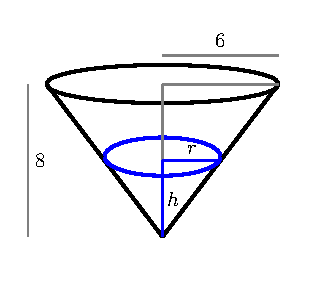
\includegraphics{figures/3_5_Act1Soln.eps}
	\end{center}
	\item Observe that the right triangle with legs of length $h$ and $r$ is similar to the right triangle with legs of length $8$ and $6$, respectively, based on how the water assumes the shape of the tank, and thus $\frac{r}{h} = \frac{6}{8}$, so that $r = \frac{3}{4}h$.
	\item Since the water in the tank always takes the shape of a circular cone, the volume of water in the tank at time $t$ is given by $V = \frac{1}{3}\pi r^2 h$.  Because we have established that $r = \frac{3}{4}h$, it follows that
	$$V = \frac{1}{3}\pi \left( \frac{3}{4}h \right)^2 h = \frac{3}{16} \pi h^3.$$ 
	\item Differentiating with respect to $t$, we now find
	$$\frac{dV}{dt} = \frac{1}{16} \pi h^2 \frac{dh}{dt},$$
	which relates the rates of change of $V$ and $h$.
	\item It is given in the problem setting that water is entering the tank at a rate of 4 cubic feet per minute, hence $\frac{dV}{dt} = 4$, and we are interested in the rate of change of the water's depth when $h = 3$.  Substituting these values into the equation that relates $\frac{dV}{dt}$ and $\frac{dh}{dt}$, we find that
	$$4 =  \frac{1}{16} \pi 3^2 \left. \frac{dh}{dt} \right|_{h=3},$$
	so that $\left. \frac{dh}{dt} \right|_{h=3} = \frac{64}{9\pi} \approx 2.2635$ feet per minute.
\ea
\end{activitySolution}
\aftera % ACTIVITY

Recognizing familiar geometric configurations is one way that we relate the changing quantities in a given problem.  For instance, while the problem in Activity~\ref{A:3.1.1} is centered on a conical tank, one of the most important observations is that there are two key right triangles present.  In another setting, a right triangle might be indicative of an opportunity to take advantage of the Pythagorean Theorem to relate the legs of the triangle.  But in the conical tank, the fact that the water at any time fills a portion of the tank in such a way that the ratio of radius to depth is constant turns out to be the most important relationship with which to work.  That enables us to write $r$ in terms of $h$ and reduce the overall problem to one where the volume of water depends simply on $h$, and hence to subsequently relate $\frac{dV}{dt}$ and $\frac{dh}{dt}$.  In other situations where a changing angle is involved, a right triangle may offer the opportunity to find relationships among various parts of the triangle using trigonometric functions.

\begin{activity} \label{A:3.1.2}  A television camera is positioned $4000$ feet from the base of a rocket launching pad.  The angle of elevation of the camera has to change at the correct rate in order to keep the rocket in sight.  In addition, the auto-focus of the camera has to take into account the increasing distance between the camera and the rocket.  We assume that the rocket rises vertically.  (A similar problem is discussed and pictured dynamically at \href{http://gvsu.edu/s/9t}{\texttt{http://gvsu.edu/s/9t}}.  Exploring the applet at the link will be helpful to you in answering the questions that follow.)
\ba
	\item Draw a figure that summarizes the given situation.  What parts of the picture are changing?  What parts are constant?  Introduce appropriate variables to represent the quantities that are changing.
	\item Find an equation that relates the camera's angle of elevation to the height of the rocket, and then find an equation that relates the instantaneous rate of change of the camera's elevation angle to the instantaneous rate of change of the rocket's height (where all rates of change are with respect to time).
	\item Find an equation that relates the distance from the camera to the rocket to the rocket's height, as well as an equation that relates the instantaneous rate of change of distance from the camera to the rocket to the instantaneous rate of change of the rocket's height (where all rates of change are with respect to time).
	\item Suppose that the rocket's speed is $600$ ft/sec at the instant it has risen $3000$ feet.  How fast is the distance from the television camera to the rocket changing at that moment?  If the camera is following the rocket, how fast is the camera's angle of elevation changing at that same moment?
	\item If from an elevation of $3000$ feet onward the rocket continues to rise at $600$ feet/sec, will the rate of change of distance with respect to time be greater when the elevation is $4000$ feet than it was at $3000$ feet, or less?  Why?  
\ea
\end{activity}
\begin{smallhint}
\ba
	\item Let $\theta$ represent the camera angle and note that one leg of the right triangle is constant.  Which two are changing?
	\item Think trigonometrically.
	\item Think like Pythagoras.
	\item Use the facts that $h = 3000$ and $\frac{dh}{dt} = 600$ in your preceding work.
	\item You can answer this question intuitively or by changing the value of $h$ in your work in (d).
\ea
\end{smallhint}
\begin{bighint}
\ba
	\item Let $\theta$ represent the camera angle and note that one leg of the right triangle is constant.  Note that both the hypotenuse and the vertical leg of the triangle are changing as the rocket rises.
	\item Think trigonometrically; which trigonometric function will only use the rocket's height along with the constant value of 4000?
	\item Use the Pythagorean Theorem to relate the three sides of the right triangle.
	\item Use the facts that $h = 3000$ and $\frac{dh}{dt} = 600$ in your preceding work.  Note that these only apply after you have completed the work of differentiation, because $h$ is changing, not constant at 3000 feet.
	\item You can answer this question intuitively or by changing the value of $h$ in your work in (d).
\ea
\end{bighint}
\begin{activitySolution}
\ba
	\item Letting $\theta$ be the camera's elevation angle, $h$ the rocket's height, and $z$ the distance from the camera to the rocket, we have the following situation at a given point in time:
	\begin{center}
	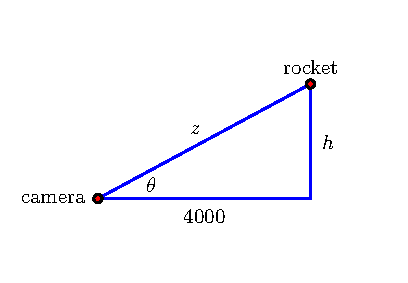
\includegraphics{figures/3_5_Act2Soln.eps}
	\end{center}
	\item To relate $\theta$ and $h$, observe that the tangent function is a good choice, since $\tan(\theta) = \frac{h}{4000}$, so that
	$$h = 4000 \tan(\theta).$$
	Differentiating implicitly with respect to $t$, we find that
	$$\frac{dh}{dt} = 4000 \sec^2 (\theta) \frac{d\theta}{dt}.$$
	\item To relate $z$ and $h$, the Pythagorean Theorem is natural to consider.  By this famous result, 
	$$h^2 + 4000^2 = z^2.$$
	Differentiating both sides implicitly with respect to $t$, it follows
	$$2h \frac{dh}{dt} = 2z \frac{dz}{dt},$$
	and thus $h \frac{dh}{dt} = z \frac{dz}{dt}.$
	\item Using the given fact that the rocket's speed is 600 ft/sec at the instant it has risen 3000 feet, we know that $\left. \frac{dh}{dt} \right|_{h=3000} = 600$.  Note further in the triangle that when $h = 3000$, it follows $z = 5000$, since the base leg of the triangle is constant at 4000, by using the Pythagorean Theorem.  Substituting this information from the instant $h = 3000$ into the equation that relates the rates of change of $z$ and $h$ found in (c), we find that 
	$$2 \cdot 3000 \cdot 600 = 2 \cdot 5000 \cdot \left. \frac{dz}{dt} \right|_{h=3000}.$$
	Solving for $\left. \frac{dz}{dt} \right|_{h=3000}$ we have 
	$$\left. \frac{dz}{dt} \right|_{h=3000} = \frac{1800}{5} = 360 \ \mbox{feet/sec}.$$
	
	To answer the question about how fast the camera angle is changing, we use the same information but now in the equation we found in (b) that relates the rates of change of $\theta$ and $h$:
	$$\frac{dh}{dt} = 4000 \sec^2 (\theta) \frac{d\theta}{dt}.$$
	Observe that when $h = 3000$, in the 3000-4000-5000 right triangle, it follows that $\cos(\theta) = \frac{4}{5}$, so $\sec(\theta) = \frac{5}{4}$.  Thus, using the instantaneous information,
	$$600 = 4000 \cdot \frac{25}{16} \left. \frac{d\theta}{dt} \right|_{h=3000},$$
	and thus
	$$ \left. \frac{d\theta}{dt} \right|_{h=3000} = \frac{6 \cdot 16}{40 \cdot 25} = \frac{12}{125},$$
	which is measured in radians per second.
	\item Recalling that $2h \frac{dh}{dt} = 2z \frac{dz}{dt}$, it follows that 
	$$\frac{dz}{dt} = \frac{h}{z} \frac{dh}{dt}.$$
	Using this equation when $h = 3000$ and $\frac{dh}{dt} = 600$ led us to conclude that $\left. \frac{dz}{dt} \right|_{h=3000} = \frac{3}{5} \cdot 600 = 360 \ \mbox{feet/sec}$.  If we instead use $h = 4000$, it follows that $z = 4000\sqrt{2}$, so that
	$$\left. \frac{dz}{dt} \right|_{h=4000} = \frac{4}{4\sqrt{2}} \cdot 600 \approx 424.26 \ \mbox{feet/sec}.$$
	Indeed, $\frac{dz}{dt}$ is an increasing function of $h$, provided that $\frac{dh}{dt}$ is constant, because we can write $h^2 + 4000^2 = z^2$, so $z = \sqrt{h^2 + 4000^2}$, making
	$$\frac{dz}{dt} = \frac{h}{\sqrt{h^2 + 4000^2}} \frac{dh}{dt} = \frac{h}{\sqrt{h^2 + 4000^2}} 600.$$
	It is straightforward to verify that $\frac{h}{\sqrt{h^2 + 4000^2}}$ is an increasing function of $h$.
\ea
\end{activitySolution}
\aftera





 % ACTIVITY

In addition to being able to find instantaneous rates of change at particular points in time, we are often able to make more general observations about how particular rates themselves will change over time.  For instance, when a conical tank (point down) is filling with water at a constant rate, we naturally intuit that the depth of the water should increase more slowly over time.  Note how carefully we need to speak:  we mean to say that while the depth, $h$, of the water is increasing, its rate of change $\frac{dh}{dt}$ is decreasing (both as a function of $t$ and as a function of $h$).  These observations may often be made by taking the general equation that relates the various rates and solving for one of them, and doing this without substituting any particular values for known variables or rates.  For instance, in the conical tank problem in Activity~\ref{A:3.1.1}, we established that 
$$\frac{dV}{dt} = \frac{1}{16} \pi h^2 \frac{dh}{dt},$$
and hence
$$\frac{dh}{dt} = \frac{16}{\pi h^2} \frac{dV}{dt}.$$
Provided that $\frac{dV}{dt}$ is constant, it is immediately apparent that as $h$ gets larger, $\frac{dh}{dt}$ will get smaller, while always remaining positive.  Hence, the depth of the water is increasing at a decreasing rate.

\begin{activity} \label{A:3.1.3}  As pictured in the applet at~\href{http://gvsu.edu/s/9q}{\texttt{http://gvsu.edu/s/9q}}, a skateboarder who is $6$ feet tall rides under a $15$ foot tall lamppost at a constant rate of $3$ feet per second.  We are interested in understanding how fast his shadow is changing at various points in time.
\ba
	\item Draw an appropriate right triangle that represents a snapshot in time of the skateboarder, lamppost, and his shadow.  Let $x$ denote the horizontal distance from the base of the lamppost to the skateboarder and $s$ represent the length of his shadow.  Label these quantities, as well as the skateboarder's height and the lamppost's height on the diagram.
	\item Observe that the skateboarder and the lamppost represent parallel line segments in the diagram, and thus similar triangles are present.  Use similar triangles to establish an equation that relates $x$ and $s$.
	\item Use your work in (b) to find an equation that relates $\frac{dx}{dt}$ and $\frac{ds}{dt}$.
	\item At what rate is the length of the skateboarder's shadow increasing at the instant the skateboarder is $8$ feet from the lamppost?
	\item As the skateboarder's distance from the lamppost increases, is his shadow's length increasing at an increasing rate, increasing at a decreasing rate, or increasing at a constant rate?
	\item Which is moving more rapidly:  the skateboarder or the tip of his shadow?  Explain, and justify your answer.
\ea
\end{activity}
\begin{smallhint}
\ba
	\item Note that the lengths of the legs of the right triangle will be $15$ for the vertical one and $x + s$ for the horizontal one.
	\item The small triangle formed by the skateboarder and his shadow, with legs $6$ and $s$ is similar to the large triangle that has the lamppost as one of its legs.
	\item Simplify the equation in (b) as much as possible before differentiating implicitly with respect to $t$.
	\item Find $\left. \frac{ds}{dt} \right|_{x=8}$.
	\item Does the equation that relates $\frac{dx}{dt}$ and $\frac{ds}{dt}$ involve $x$?  Is $\frac{dx}{dt}$ changing or constant?
	\item Let $y$ represent the location of the tip of the shadow, so that $y = x + s$.
\ea
\end{smallhint}
\begin{bighint}
\ba
	\item Note that the lengths of the legs of the overall right triangle will be $15$ for the vertical one and $x + s$ for the horizontal one, with a smaller right triangle with legs of length 6 and $s$.
	\item The small triangle formed by the skateboarder and his shadow, with legs $6$ and $s$ is similar to the large triangle that has legs of length $15$ and $x + s$.  Remember that the ratios of the lengths of legs of similar triangles must be equal.
	\item Simplify the equation in (b) as much as possible before differentiating implicitly with respect to $t$.
	\item Find $\left. \frac{ds}{dt} \right|_{x=8}$.  Your answer should not depend on the value of $x$.
	\item Does the equation that relates $\frac{dx}{dt}$ and $\frac{ds}{dt}$ involve $x$?  Is $\frac{dx}{dt}$ changing or constant?
	\item Let $y$ represent the location of the tip of the shadow, so that $y = x + s$.  Observe that you can then write $\frac{dy}{dt}$ in terms of $\frac{dx}{dt}$ and $\frac{ds}{dt}$.
\ea
\end{bighint}
\begin{activitySolution}
\ba
	\item The given information leads us to construct the following diagram:
	\begin{center}
	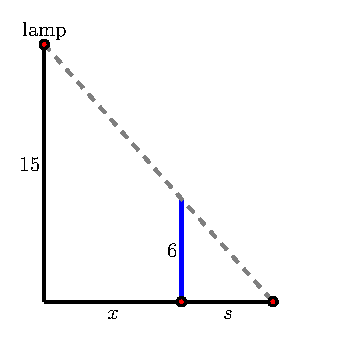
\includegraphics{figures/3_5_Act3Soln.eps}
	\end{center}
	\item The small triangle formed by the skateboarder and his shadow, with legs of length $6$ and $s$ is similar to the large triangle that has the lamppost as one of its legs (length 15) and horizontal leg of length $x + s$.  Because the ratios of the lengths of the legs of these two triangles is equal, we have
	$$\frac{s}{6} = \frac{s+x}{15}.$$  
	Simplifying, we have $15s = 6s + 6x$, so that $9s = 2x$, or most simply, $3s = 2x$.
	\item Differentiating with respect to $t$, it is immediate that $3 \frac{ds}{dt} = 2\frac{dx}{dt}$.
	\item Since $\frac{ds}{dt} = \frac{2}{3} \frac{dx}{dt}$, and $\frac{dx}{dt} = 3$, it follows $\frac{ds}{dt} = 2$ for every value of $t$ (and $x$).  Thus, $\left. \frac{ds}{dt} \right|_{x=8} = 2$ feet per second.
	\item Because $\frac{ds}{dt}$ is constant, the shadow's length is increasing at a constant rate (irrespective of the distance from the skateboarder to the lamppost). 
	\item Let $y$ represent the location of the tip of the shadow, so that $y = x + s$.  Observe that we can now compute $\frac{dy}{dt}$ in terms of $\frac{dx}{dt}$ and $\frac{ds}{dt}$, with $\frac{dy}{dt} = \frac{dx}{dt} + \frac{ds}{dt} = 3 + 2 = 5$ feet/sec, and hence the tip of the shadow is moving more rapidly than the skateboarder himself.
\ea
\end{activitySolution}
\aftera





 % ACTIVITY

As we progress further into related rates problems, less direction will be provided.  In the first three activities of this section, we have been provided with guided instruction to build a solution in a step by step way.  For the closing activity and the following exercises, most of the detailed work is left to the reader.

\begin{activity} \label{A:3.1.4}  
A baseball diamond is $90'$ square.  A batter who hits a ball along the third base line runs to first base.  At what rate is the distance between the ball and first base changing when the ball is halfway to third base, if at that instant the ball is traveling $100$ feet/sec?  At what rate is the distance between the ball and the runner changing at the same instant, if at the same instant the runner is $1/8$ of the way to first base running at $30$ feet/sec?
\end{activity}
\begin{smallhint}
Let $x$ denote the position of the ball along the third base line at time $t$, and $z$ the distance from the ball to first base.  Note that the basepaths meet at 90 degree angles.
\end{smallhint}
\begin{bighint}
Let $x$ denote the position of the ball along the third base line at time $t$, and $z$ the distance from the ball to first base.  Note that the basepaths meet at 90 degree angles.  Find a right triangle in which you can use the Pythagorean Theorem.  When including the runner for the second question, let $r$ denote the runner's position at time $t$, and again work with a key right triangle.
\end{bighint}
\begin{activitySolution}
We let $x$ denote the position of the ball at time $t$ and $z$ the distance from the ball to first base, as pictured below.
\begin{center}
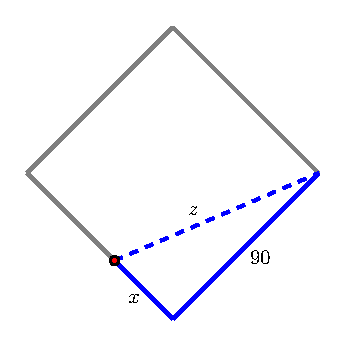
\includegraphics{figures/3_5_Act4Soln1.eps}
\end{center}
By the Pythagorean Theorem, we know that $x^2 + 90^2 = z^2$; differentiating with respect to $t$, we have
$$2x\frac{dx}{dt} = 2z\frac{dz}{dt}.$$
At the instant the ball is halfway to third base, we know $x = 45$ and $\left. \frac{dx}{dt} \right|_{x = 45} = 100$.  Moreover, by Pythagoras, $z^2 = 90^2 + 45^2$, so $z = 45\sqrt{5}$.  Thus,
$$2 \cdot 45 \cdot 100 = 2 \cdot 45 \sqrt{5} \cdot \left. \frac{dz}{dt} \right|_{x = 45},$$
so 
$$\left. \frac{dz}{dt} \right|_{x = 45} = \frac{100}{\sqrt{5}} \approx 44.7214 \ \mbox{feet/sec}.$$

For the second question, we still let $x$ represent the ball's position at time $t$, but now we introduce $r$ as the runner's position at time $t$ and let $s$ be the distance between the runner and the ball.  In this setting, as seen in the diagram below,
\begin{center}
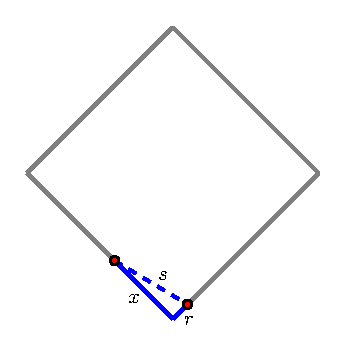
\includegraphics{figures/3_5_Act4Soln2.eps}
\end{center}
$x$, $r$, and $s$ form the sides of a right triangle, so that
$$x^2 + r^2 = s^2,$$
by the Pythagorean Theorem.  Differentiating each side with respect to $t$, it follows that the three rates of change are related by the equation
$$2x \frac{dx}{dt} + 2r \frac{dr}{dt} = 2s \frac{ds}{dt}.$$
We are given that at the instant $x = 45$, $r = \frac{90}{8}$, so by Pythagoras, $s = \frac{45}{4}\sqrt{17}$.  In addition, at this same instant we know that $\left. \frac{dx}{dt} \right|_{x = 45} = 100$ and $\left. \frac{dr}{dt} \right|_{x = 45} = 30$.  Applying this information,
$$2 \cdot 45 \cdot 100 + 2 \cdot \frac{45}{4} \cdot 30 = 2 \cdot \frac{45}{4}\sqrt{17} \cdot \left. \frac{ds}{dt} \right|_{x = 45}$$
and therefore
$$\left. \frac{ds}{dt} \right|_{x = 45} = \frac{430}{\sqrt{17}} \approx 104.2903 \ \mbox{feet/sec}.$$
\end{activitySolution}
\aftera % ACTIVITY

%-------------
% SUMMARY
%-------------
\begin{summary}
\item When two or more related quantities are changing as implicit functions of time, their rates of change can be related by implicitly differentiating the equation that relates the quantities themselves.  For instance, if the sides of a right triangle are all changing as functions of time, say having lengths $x$, $y$, and $z$, then these quantities are related by the Pythagorean Theorem: $x^2 + y^2 = z^2$.  It follows by implicitly differentiating with respect to $t$ that their rates are related by the equation
$$2x \frac{dx}{dt} + 2y\frac{dy}{dt} = 2z \frac{dz}{dt},$$ 
so that if we know the values of $x$, $y$, and $z$ at a particular time, as well as two of the three rates, we can deduce the value of the third.
\end{summary}

\clearpage

%--------------
% EXERCISES
%--------------
\begin{adjustwidth*}{}{-2.25in}
\textbf{{\large Exercises}}
\setlength{\columnsep}{25pt}
\begin{multicols*}{2}
\noindent Terms and Concepts \small
\begin{enumerate}[1)]
\item T/F: Implicit differentiation is often used when solving ``related rates'' type problems.
\end{enumerate} 

\noindent {\normalsize Problems} \small

\begin{enumerate}[1),resume]
\item Water flows onto a flat surface at a rate of $5$ cm$^3$/s forming a circular puddle $10$ mm deep. How fast is the radius growing when the radius is:
	\begin{enumerate}
	\item		$1$ cm?
	\item		$10$ cm?
	\item		$100$ cm?
	\end{enumerate}
	
\item A circular balloon is inflated with air flowing at a rate of $10$ cm$^3$/s. How fast is the radius of the balloon increasing when the radius is:
	\begin{enumerate}
	\item		$1$ cm?
	\item		$10$ cm?
	\item		$100$ cm?
	\end{enumerate}
	
\item Consider the traffic situation introduced in Example~\ref{Ex:3.1.Eg1}. How fast is the ``other car'' traveling if the officer and the other car are each $1/2$ mile from the intersection, the officer is traveling $50$ mph, and the radar reading is $70$ mph?

\item Consider the traffic situation introduced in Example \ref{Ex:3.1.Eg1}. How fast is the ``other car'' traveling if the officer and the other car are each $1$ mile from the intersection, the officer is traveling $60$ mph, and the radar reading is $80$ mph?

\item \label{exer:04_02_ex_07}An F-22 aircraft is flying at $500$ mph with an elevation of  $10,000$ ft on a straight--line path that will take it directly over an anti--aircraft gun. 

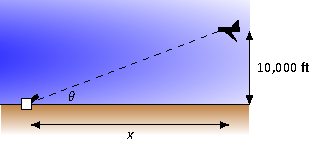
\includegraphics{figures/fig04_02_ex_07}

How fast must the gun be able to turn to accurately track the aircraft when the plane is:
\begin{enumerate}
\item	$1$ mile away?
\item	$1/5$ mile away?
\item	Directly overhead?
\end{enumerate}

\item An F-$22$ aircraft is flying at $500$ mph with an elevation of  $100$ ft on a straight--line path that will take it directly over an anti--aircraft gun as in Exercise \ref{exer:04_02_ex_07} (note the lower elevation here).

How fast must the gun be able to turn to accurately track the aircraft when the plane is:
\begin{enumerate}
\item	$1000$ feet away?
\item	$100$ feet away?
\item	Directly overhead?
\end{enumerate}

\item A $24$ ft. ladder is leaning against a house while the base is pulled away at a constant rate of $1$ ft/s.

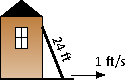
\includegraphics{figures/fig04_02_ex_09}

At what rate is the top of the ladder sliding down the side of the house when the base is:
\begin{enumerate}
\item	$1$ foot from the house?
\item	$10$ feet from the house?
\item	$23$ feet from the house?
\item	$24$ feet from the house?
\end{enumerate}

\item A boat is being pulled into a dock at a constant rate of $30$ ft/min by a winch located $10$ ft above the deck of the boat.

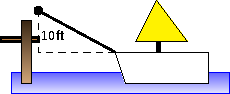
\includegraphics{figures/fig04_02_ex_10}

At what rate is the boat approaching the dock when the boat is:
\begin{enumerate}
\item	$50$ feet out?
\item	$15$ feet out?
\item	$1$ foot from the dock?
\item	What happens when the length of rope pulling in the boat is less than 10 feet long?
\end{enumerate}

\item An inverted cylindrical cone, $20$ ft deep and $10$ ft across at the top, is being filled with water at a rate of $10$ ft$^3$/min. At what rate is the water rising in the tank when the depth of the water is:
\begin{enumerate}
\item	1 foot?
\item	10 feet?
\item	19 feet?
\end{enumerate}
How long will the tank take to fill when starting at empty?

\item A hot air balloon lifts off from ground rising vertically. From $100$ feet away, a $5$' woman tracks the path of the balloon. When her sightline with the balloon makes a $45^\circ$ angle with the horizontal, she notes the angle is increasing at about $5^\circ$/min. 
\begin{enumerate}
\item		What is the elevation of the balloon?
\item		How fast is it rising?
\end{enumerate}



\end{enumerate}

%------------------------------------------
% END OF EXERCISES ON FIRST PAGE
%------------------------------------------
\end{multicols*}
\end{adjustwidth*}

\clearpage

\begin{adjustwidth*}{}{-2.25in}
\setlength{\columnsep}{25pt}
\begin{multicols*}{2}\small

\begin{enumerate}[1),start=12]

\item \label{exer:04_02_ex_12}A rope, attached to a weight, goes up through a pulley at the ceiling and back down to a worker. The man holds the rope at the same height as the connection point between rope and weight.

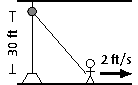
\includegraphics[scale=1.25]{figures/fig04_02_ex_12}

Suppose the man stands directly next to the weight (i.e., a total rope length of $60$ ft) and begins to walk away at a rate of $2$ ft/s. How fast is the weight rising when the man has walked:
\begin{enumerate}
\item	$10$ feet?
\item	$40$ feet?
\end{enumerate}
How far must the man walk to raise the weight all the way to the pulley?

\item Consider the situation described in Exercise \ref{exer:04_02_ex_12}. Suppose the man starts $40$ ft from the weight and begins to walk away at a rate of $2$ ft/s. 
\begin{enumerate}
\item	How long is the rope?
\item	How fast is the weight rising after the man has walked $10$ feet?
\item	How fast is the weight rising after the man has walked $40$ feet?
\item	How far must the man walk to raise the weight all the way to the pulley?
\end{enumerate}

\item A company that produces landscaping materials is dumping sand into a conical pile. The sand is being poured at a rate of $5$ ft$^3$/sec; the physical properties of the sand, in conjunction with gravity, ensure that the cone's height is roughly $2/3$ the length of the diameter of the circular base. 

How fast is the cone rising when it has a height of $30$ feet?

\item A baseball diamond is a square with sides $90$ feet long.  Suppose a baseball player is advancing from second to third base at the rate of $24$ feet per second, and an umpire is standing on home plate.  Let  $\theta$ be the angle between the third baseline and the line of sight from the umpire to the runner.  How fast is $\theta$ changing when the runner is $30$ feet from third base?
	
\item Sand is being dumped off a conveyor belt onto a pile in such a way that the pile forms in the shape of a cone whose radius is always equal to its height.  Assuming that the sand is being dumped at a rate of $10$ cubic feet per minute, how fast is the height of the pile changing when there are $1000$ cubic feet on the pile?
	
\item A swimming pool is $60$ feet long and $25$ feet wide. Its depth varies uniformly from $3$ feet at the shallow end to $15$ feet at the deep end, as shown below.
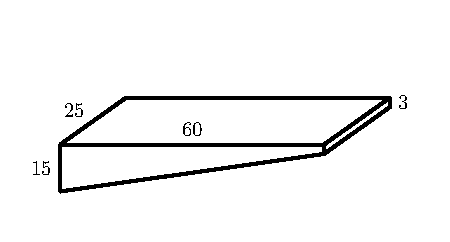
\includegraphics{figures/3_5_Ez3.eps}
Suppose the pool has been emptied and is now being filled with water at a rate of $800$ cubic feet per minute. At what rate is the depth of water (measured at the deepest point of the pool) increasing when it is $5$ feet deep at that end?  Over time, describe how the depth of the water will increase:  at an increasing rate, at a decreasing rate, or at a constant rate.  Explain.

\end{enumerate}

%---------------------------------------------
% END OF EXERCISES ON SECOND PAGE
%---------------------------------------------
\end{multicols*}
\end{adjustwidth*}

\afterexercises 

\cleardoublepage